\documentclass{beamer}
\usepackage{amsmath,amssymb}
\usepackage{graphicx}
\usepackage{siunitx}
\sisetup{per-mode=symbol}
\usepackage{gvv}
\usepackage{listings}
\usepackage{xcolor}

% Code style
\lstset{
  basicstyle=\ttfamily\scriptsize,
  breaklines=true,
  frame=single,
  numbers=left,
  numberstyle=\tiny,
  keywordstyle=\color{blue},
  commentstyle=\color{green!50!black},
  stringstyle=\color{red!60!black},
  showstringspaces=false
}

\title{Matrix 4.8.11}
\author{ai25btech11015 -- M Sai Rithik}
\date{}

\begin{document}

\frame{\titlepage}

\begin{frame}
\frametitle{Question}
Find the vector equation of the plane determined by the points
\[
A(3,-1,2),\quad B(5,2,4),\quad C(-1,-1,6),
\]
and hence find the distance of this plane from the origin.  

\end{frame}

\begin{frame}
\frametitle{Step 1: Position vectors}
\begin{equation}
\Vec{A} = \myvec{3 \\ -1 \\ 2},\quad
\Vec{B} = \myvec{5 \\ 2 \\ 4},\quad
\Vec{C} = \myvec{-1 \\ -1 \\ 6}.
\end{equation}
\pause
\begin{equation}
\Vec{B}-\Vec{A} = \myvec{2 \\ 3 \\ 2},\quad
\Vec{C}-\Vec{A} = \myvec{-4 \\ 0 \\ 4}.
\end{equation}
\end{frame}

\begin{frame}
\frametitle{Step 2: Normal via cross product}
\begin{equation}
(\Vec{B}-\Vec{A}) \times (\Vec{C}-\Vec{A})
= \myvec{
  \mydet{\myvec{3\\2} & \myvec{0\\4}} \\[1ex]
  \mydet{\myvec{2\\2} & \myvec{-4\\4}} \\[1ex]
  \mydet{\myvec{2\\3} & \myvec{-4\\0}}
}.
\end{equation}
\pause
\begin{equation}
= \myvec{12 \\ 16 \\ 12}.
\end{equation}
\pause
Simplify by dividing through $4$:
\begin{equation}
\Vec{N} = \myvec{3 \\ -4 \\ 3}.
\end{equation}
\end{frame}

\begin{frame}
\frametitle{Step 3: Finding place Eqn}
Using $\Vec{A}$:
\begin{equation}
d = \Vec{N}^{\!\top}\Vec{A}
= \begin{pmatrix}3 & -4 & 3\end{pmatrix}\myvec{3\\-1\\2}.
\end{equation}
\pause
\begin{equation}
d = 9 + 4 + 6 = 19.
\end{equation}
\pause
Equation of plane:
\begin{equation}
\Vec{N}^{\!\top}x = 19.
\end{equation}
\end{frame}

\begin{frame}
\frametitle{Step 4: Normalize to $N^\top x = 1$}
\begin{equation}
\widetilde{\Vec{N}} = \frac{1}{19}\Vec{N}
= \myvec{\tfrac{3}{19}\\[4pt]-\tfrac{4}{19}\\[4pt]\tfrac{3}{19}}.
\end{equation}
\pause
\begin{equation}
\boxed{\;\widetilde{\Vec{N}}^{\!\top} x = 1\;}
\end{equation}
\end{frame}

\begin{frame}
\frametitle{Step 5: Distance from origin}
For $\widetilde{\Vec{N}}^{\!\top}x = 1$:
\begin{equation}
D = \frac{|1|}{\|\widetilde{\Vec{N}}\|}.
\end{equation}
\pause
\begin{equation}
\|\Vec{N}\| = \sqrt{3^2+(-4)^2+3^2} = \sqrt{34}.
\end{equation}
\pause
\begin{equation}
\|\widetilde{\Vec{N}}\| = \frac{\|\Vec{N}\|}{19}.
\end{equation}
\pause
\begin{equation}
D = \frac{19}{\sqrt{34}} \approx 3.260.
\end{equation}
\end{frame}

\begin{frame}
\frametitle{Final Answer}
\begin{equation}
\boxed{\;\widetilde{\Vec{N}}^{\!\top}x = 1,\quad
\widetilde{\Vec{N}} = \myvec{\tfrac{3}{19}\\[4pt]-\tfrac{4}{19}\\[4pt]\tfrac{3}{19}}}
\end{equation}
\begin{equation}
\boxed{\;D = \tfrac{19}{\sqrt{34}} \;\approx 3.260\;}
\end{equation}
\end{frame}
\begin{frame}
\begin{figure}[h!]
    \centering
    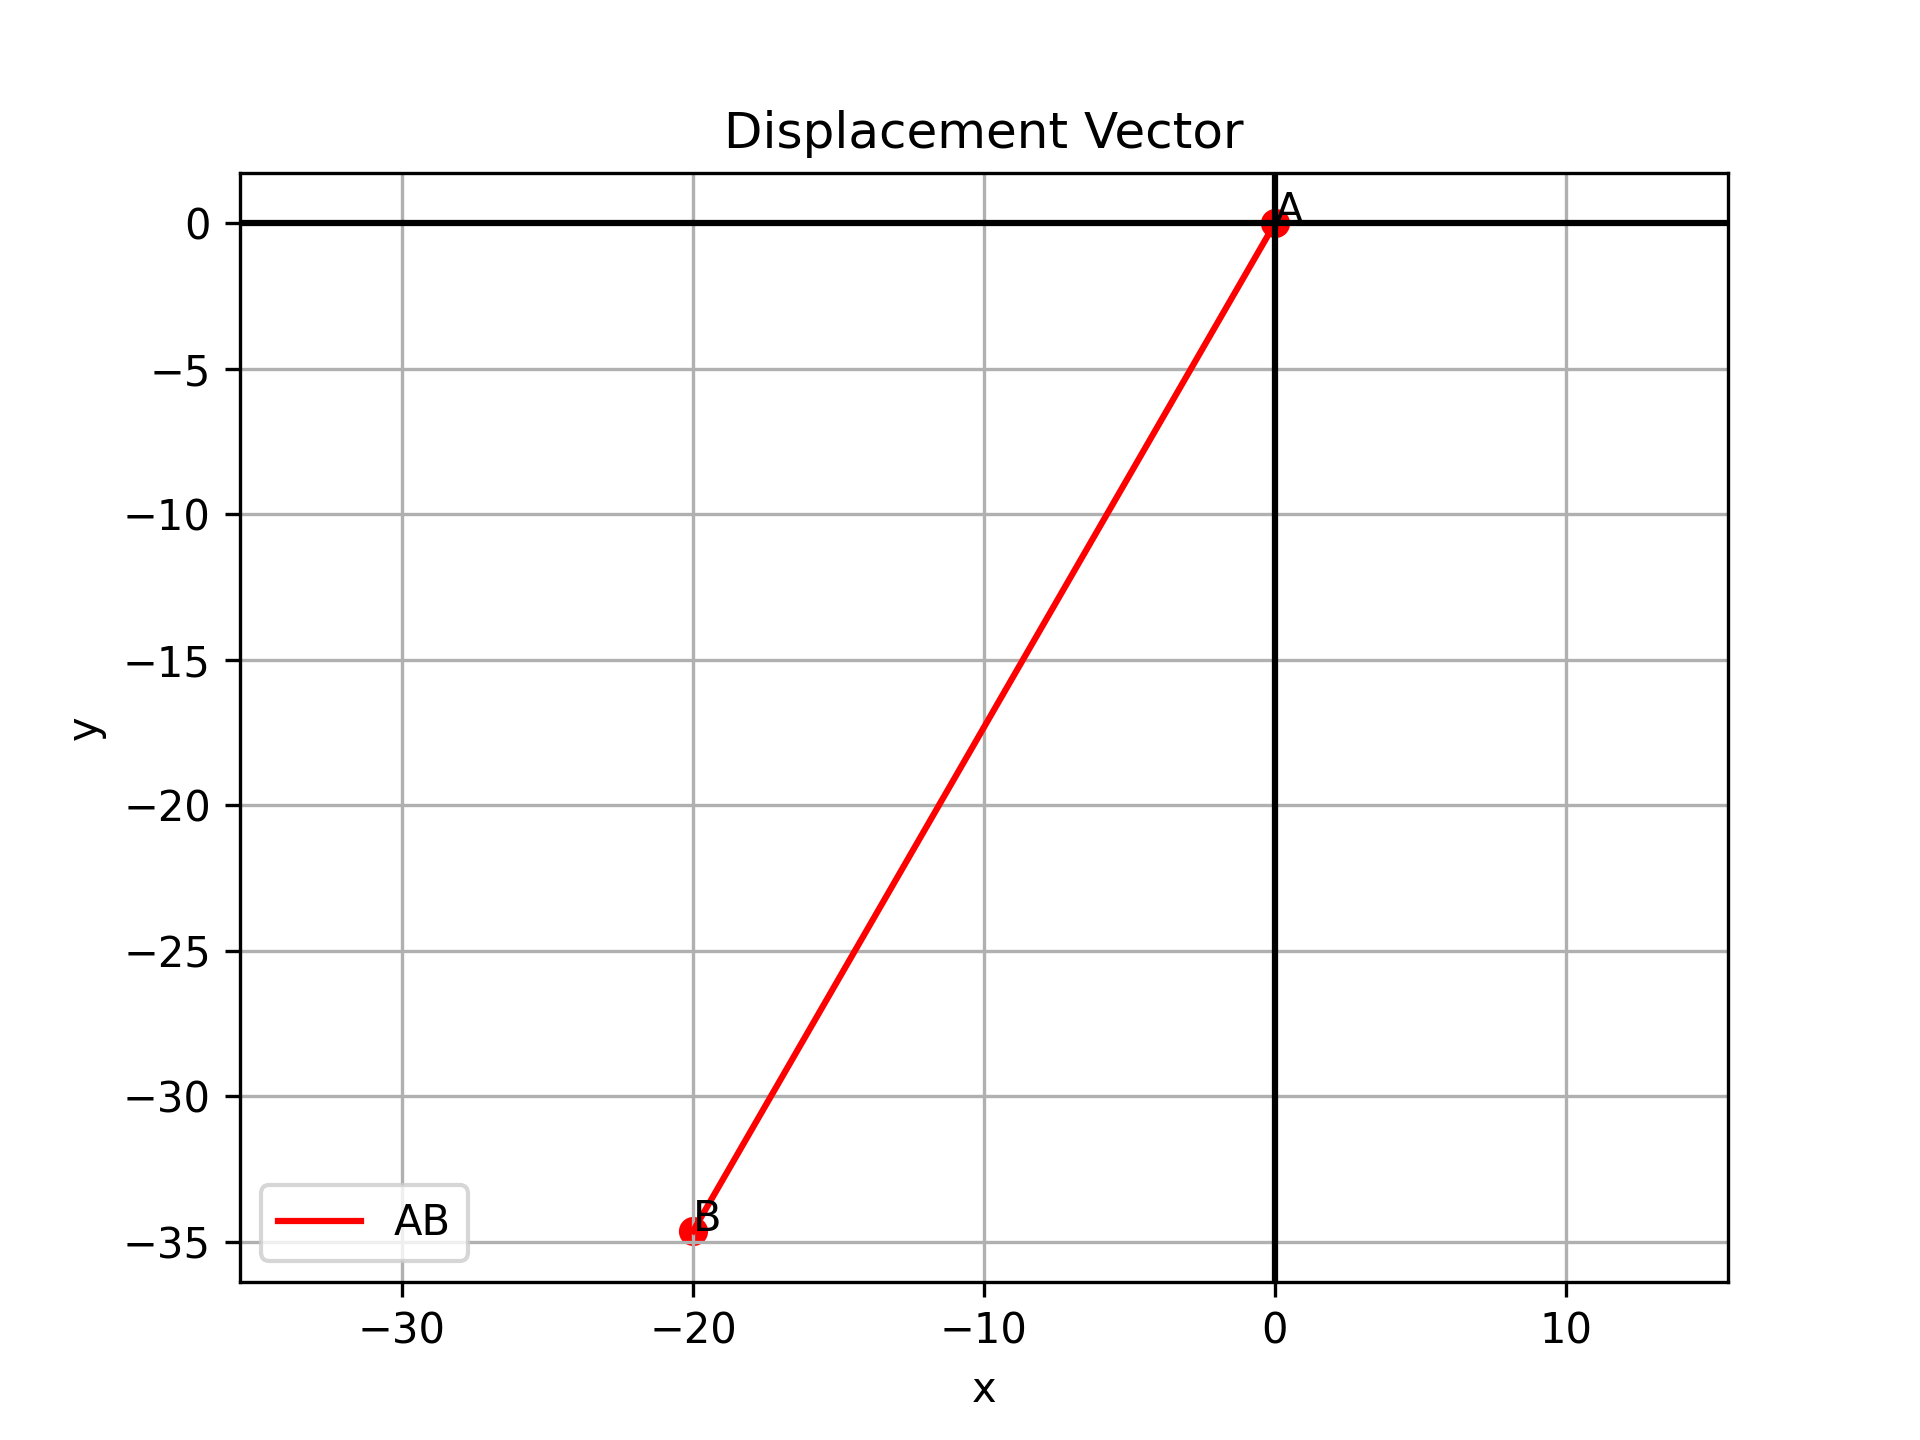
\includegraphics[width=0.65\linewidth]{figs/fig.png}
    \caption{}
\end{figure}
\end{frame}

\end{document}
